% !TeX root = ../main.tex

\chapter{卷积：LTI 系统的时域核心}
\label{chap:convolution}

卷积是 LTI 系统时域分析的主线。核心只有两句话：单位脉冲响应是系统的唯一标识；任意输入都能拆成移位脉冲的加权和。知道单位脉冲响应，就能算出任意输入的响应。

\section{LTI 系统的时域分析目标}
\label{sec:lti-time-domain-goal}

同时满足线性和时不变性的系统称为\keyterm{线性时不变系统（linear time-invariant system，LTI）}。线性允许把输入拆开，分别求响应再相加；时不变保证输入延迟多少，响应只延迟多少。于是问题归结为：已知一个基本输入的响应，能否推出任意输入的响应？

离散时间选单位脉冲 $\impulse[n]$ 作基本输入。任意序列都能写成加权、移位的单位脉冲之和。知道 $\impulse[n]\longrightarrow h[n]$，再由线性和时不变逐项叠加，就能得到总响应。

\begin{remark}[LTI 不保证因果或稳定]
  LTI 只说明线性且时不变。超前系统 $y(t)=x(t+1)$ 是 LTI，却非因果。因果性和稳定性仍要单独检查。
\end{remark}

\section{单位脉冲响应}
\label{sec:discrete-impulse-response}

\begin{definition}[单位脉冲响应]
  \label{def:discrete-impulse-response}
  离散时间 LTI 系统对单位脉冲 $\impulse[n]$ 的输出称为\keyterm{单位脉冲响应（unit impulse response）}，记作 $h[n]$：
  \begin{equation}
    \impulse[n]\longrightarrow\boxed{\text{LTI 系统}}\longrightarrow h[n].
    \label{eq:discrete-impulse-response-flow}
  \end{equation}
\end{definition}

由齐次性，输入幅度乘 $a$，响应也乘 $a$；由时不变性，输入延迟 $n_0$，响应也延迟 $n_0$。合起来：
\begin{equation}
  a\impulse[n-n_0]
  \longrightarrow\boxed{\text{同一 LTI 系统}}\longrightarrow
  a h[n-n_0].
  \label{eq:scaled-shifted-impulse-response}
\end{equation}
所以 $h[n]$ 给出了所有加权、移位脉冲的响应。\red{单位脉冲响应唯一确定 LTI 系统}：两个系统的 $h[n]$ 相同，对任意可作脉冲分解的输入就给出相同输出。

\begin{example}[缩放与移位]
  若 $\impulse[n]\longrightarrow h[n]$，则
  \[
    2\impulse[n]\longrightarrow2h[n],
    \qquad
    \impulse[n-1]\longrightarrow h[n-1].
  \]
  前者只用齐次性，后者只用时不变性。两件事同时出现时，\red{幅度与时移分别传到响应上}。
\end{example}

\begin{pitfall}[把平移方向写反]
  $\impulse[n-n_0]$ 是向右延迟 $n_0$，响应应为 $h[n-n_0]$。写成 $h[n+n_0]$ 就把延迟变成了超前。\blue{用脉冲位置核对符号}：正的 $n_0$ 应把位置从 $0$ 移到 $n_0$。
\end{pitfall}

\section{由基本响应组合有限输入的响应}
\label{sec:lti-finite-superposition}

设有限长输入已分解为
\[
  x[n]=a_1\impulse[n-n_1]+\cdots+a_m\impulse[n-n_m].
\]
由\cref{eq:scaled-shifted-impulse-response}，每一项 $a_j\impulse[n-n_j]$ 的响应是 $a_jh[n-n_j]$；再由可加性，总输出是\red{这些响应的逐点叠加}：
\begin{equation}
  y[n]=a_1h[n-n_1]+\cdots+a_mh[n-n_m].
  \label{eq:finite-lti-response-superposition}
\end{equation}
这里只用\hl{分解、移位、缩放、叠加}四步，还没有套卷积公式。

\begin{intuition}
  把 $h[n]$ 看成响应模板。输入在 $n_j$ 处有幅度 $a_j$，就复制一份向右移 $n_j$、再乘 $a_j$ 的模板；所有模板按同一输出下标对齐相加，就是最终响应。
\end{intuition}

\subsection{支撑区间}

设 $x[n]$ 的首尾非零下标为 $a_1,b_1$，$h[n]$ 的首尾非零下标为 $a_2,b_2$，则输出首尾为 $a_1+a_2$ 与 $b_1+b_2$，计算范围是
\begin{equation}
  a_1+a_2\le n\le b_1+b_2.
  \label{eq:finite-response-support}
\end{equation}
记长度 $N_1=b_1-a_1+1$、$N_2=b_2-a_2+1$，则
\begin{equation}
  N_y=N_1+N_2-1.
  \label{eq:finite-response-length}
\end{equation}
动手前先算这一步，列表范围就定了；算完再核对首尾下标，能发现漏移、错移。口诀是\hl{左端相加、右端相加}。长度按首尾之间的全部位置计数，\red{内部零样值也占位}。输出在这个范围内仍可能出现零值，那是正负抵消的结果。

\subsection{列表叠加法}

每个非零输入样值写一行：把 $h[n]$ 移位、乘上该样值。每一列对应同一个输出下标，最后逐列相加。两个长度相当的短序列，列表最省事，也能看清每个输出由哪些移位响应叠成。

例如 $x[-1]=3$，这一行写 $3h[n+1]$。若 $h[-1]=1$，该行第一个数是 $3\times1$，放在输出下标 $n=-2$。后续每个数沿输出下标依次放置；$h$ \red{内部出现零值时也占一格}。完整列表见\cref{ex:lti-response-from-impulse-response}。

\begin{pitfall}[只按表格位置相加]
  各行必须\hl{按真实下标对齐}，不能只按“第几个数”对齐。先用\cref{eq:finite-response-support} 写出输出下标，再放每一行；否则乘法全对，结果也可能整体错位。
\end{pitfall}

\section{离散时间卷积}
\label{sec:discrete-convolution}

常见题型有两种：给 $\impulse[n]\longrightarrow h[n]$，求任意输入的响应；直接给 $x[n]$ 和 $h[n]$，求卷积。做法相同，都是分解、翻转、平移、相乘、求和。

任意离散信号都按单位脉冲分解：
\[
  x[n]=\sum_{k=-\infty}^{\infty}x[k]\impulse[n-k].
\]
若同一 LTI 系统满足 $\impulse[n]\longrightarrow h[n]$，则
\[
  \impulse[n-k]\longrightarrow h[n-k],
  \qquad
  x[k]\impulse[n-k]\longrightarrow x[k]h[n-k].
\]
由可加性叠加各 $k$ 的响应：
\begin{equation}
  \boxed{
    y[n]=(x\conv h)[n]
    =\sum_{k=-\infty}^{\infty}x[k]h[n-k]
  }.
  \label{eq:discrete-convolution-sum}
\end{equation}
右端称为 $x[n]$ 与 $h[n]$ 的\keyterm{卷积和（convolution sum）}。因此，LTI 系统的输出等于\red{输入与单位脉冲响应的卷积}。

\begin{intuition}
  固定输出时刻 $n$，$x[k]h[n-k]$ 是输入样值 $x[k]$ 对该时刻的贡献。对所有 $k$ 求和，就是把每个输入脉冲激发的移位响应累加。卷积由脉冲分解和 LTI 性质直接推出。
\end{intuition}

\subsection{公式法：翻转、平移、相乘、求和}

手算时先固定一个输出下标 $n$，把 $k$ 当横轴变量：
\begin{enumerate}
  \item 写出 $x[k]$ 与 $h[k]$ 的样值和下标，$x[k]$ 保持不动。
  \item 把 $h[k]$ 关于 $k=0$ 翻转成 $h[-k]$，样值随位置一起翻。
  \item 再平移成 $h[-(k-n)]=h[n-k]$：$n>0$ 右移 $n$ 格，$n<0$ 左移 $|n|$ 格。
  \item 找\red{同一下标处的样值}，\red{逐对相乘}，把乘积相加，得到当前的 $y[n]$。
  \item $n$ 增加 $1$，$h[n-k]$ 右移一格，重新列乘积与和，直到两序列完全错开。
\end{enumerate}
\Cref{fig:discrete-convolution-operations} 把翻转和平移画在同一坐标尺度下。两序列\red{没有重叠时，输出为零}。短有限序列按首尾之间的每个整数 $n$ 依次算，内部的零输出也要写出。

核对平移位置，可以盯住 $h$ 的一个已知样值：若它原来在下标 $i$，在 $h[n-k]$ 中的位置满足 $n-k=i$，即 $k=n-i$。例如 $h[2]$ 翻转后在 $k=-2$，平移后在 $k=n-2$。\Cref{ex:lti-response-from-impulse-response} 有每次平移后的对齐图和全部乘积。

\begin{figure}[htbp]
  \centering
  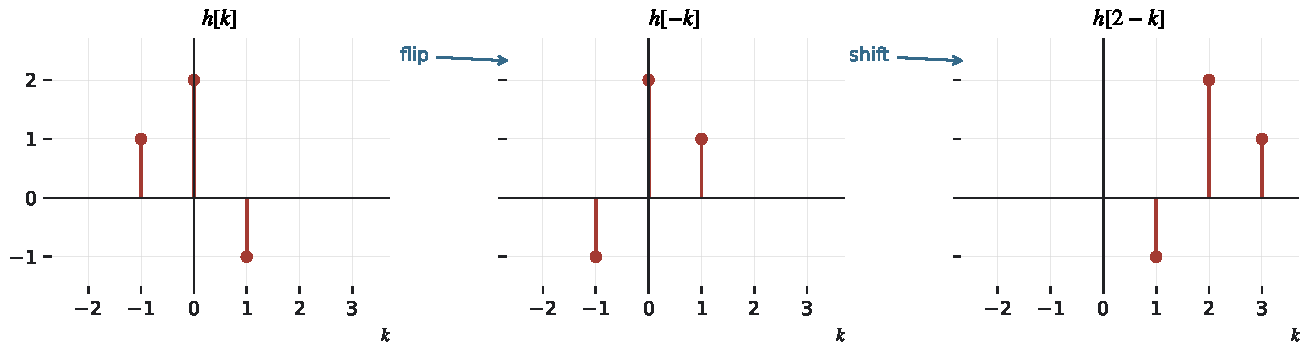
\includegraphics[width=0.92\textwidth]{04-convolution/discrete-convolution-operations.pdf}
  \caption{离散卷积中 $h[k]\to h[-k]\to h[-(k-n)]$ 的操作顺序；图中以 $n=2$ 为例。}
  \label{fig:discrete-convolution-operations}
\end{figure}

\begin{pitfall}[翻转对象或操作顺序错误]
  从\cref{eq:discrete-convolution-sum} 直接读：$x[k]$ 不动，$h[k]$ 变成 $h[n-k]$。应\hl{翻转脉冲响应}，并且\hl{先翻转、后平移}：$h[k]\to h[-k]\to h[n-k]$。先把 $h[k]$ 平移成 $h[k-n]$ 再翻转，会得到 $h[-k-n]$，方向错误。
\end{pitfall}

\begin{example}[两个等长矩形序列的卷积]
  \label{eg:rectangular-sequence-convolution}
  设
  \[
    x[n]=h[n]=\stepfun[n]-\stepfun[n-5],
  \]
  即二者在 $0\leq n\leq4$ 上为 $1$，其余为零。先定范围：左端 $0+0=0$，右端 $4+4=8$。$h[-k]$ 在 $-4\leq k\leq0$ 上为 $1$；平移后 $h[n-k]$ 在 $n-4\leq k\leq n$ 上为 $1$。$x[k]$ 不动，从 $n=0$ 开始，每次把后一行右移一格：
  \[
    \begin{array}{c|c|l}
      n & \text{重叠下标 }k & \text{乘积之和 }y[n]\\ \hline
      0 & 0 & 1\times1=1\\
      1 & 0,1 & 1\times1+1\times1=2\\
      2 & 0,1,2 & 1\times1+1\times1+1\times1=3\\
      3 & 0,1,2,3 & 1\times1+1\times1+1\times1+1\times1=4\\
      4 & 0,1,2,3,4 & 1\times1+1\times1+1\times1+1\times1+1\times1=5\\
      5 & 1,2,3,4 & 1\times1+1\times1+1\times1+1\times1=4\\
      6 & 2,3,4 & 1\times1+1\times1+1\times1=3\\
      7 & 3,4 & 1\times1+1\times1=2\\
      8 & 4 & 1\times1=1
    \end{array}
  \]
  范围外无重叠，输出为零。每个乘积都是 $1$，可以改成\hl{数重叠样点}：$n=0,\ldots,4$ 时有 $n+1$ 个，$n=5,\ldots,8$ 时有 $9-n$ 个，故
  \[
    y[n]=
    \begin{cases}
      n+1, & 0\leq n\leq4,\\
      9-n, & 5\leq n\leq8,\\
      0, & \text{其他}.
    \end{cases}
  \]
  如\cref{fig:rectangular-sequence-convolution} 所示，结果依次为 $1,2,3,4,5,4,3,2,1$；两个长度 $5$ 的序列卷积后长度为 $9$，与\cref{eq:finite-response-length} 一致。这里数的是整数样点，$0\leq k\leq4$ 共 $5$ 点，端点都算。

  \begin{figure}[htbp]
    \centering
    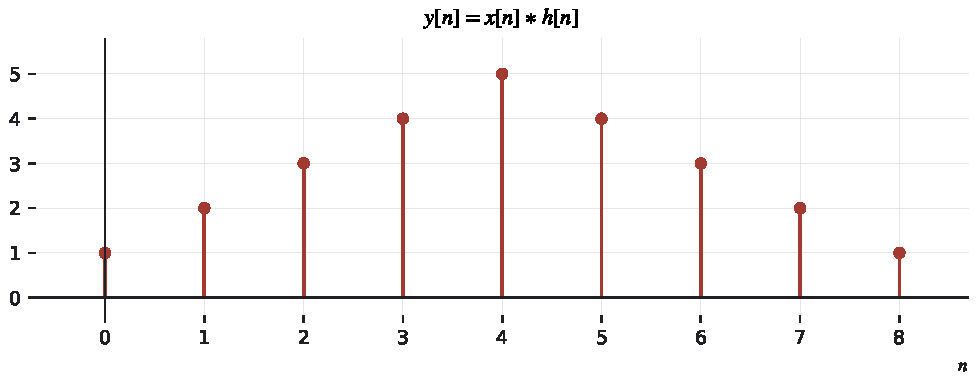
\includegraphics[width=0.78\textwidth]{04-convolution/rectangular-sequence-convolution.pdf}
    \caption{两个五点矩形序列卷积所得的三角序列。}
    \label{fig:rectangular-sequence-convolution}
  \end{figure}
\end{example}

\section{连续时间卷积}
\label{sec:continuous-convolution}

先用已知响应回顾连续时间的缩放、时移与叠加。设
\[
  p(t)=\stepfun(t)-\stepfun(t-2),\qquad
  q(t)=
  \begin{cases}
    t,&0\le t\le1,\\
    2-t,&1<t\le2,\\
    0,&\text{其他},
  \end{cases}
\]
且已知 $p(t)\longrightarrow\boxed{\text{LTI 系统}}\longrightarrow q(t)$。
宽度为 $2$ 的矩形延迟或放大时，三角响应作同样变化：
\[
  2p(t)\longrightarrow2q(t),\qquad
  p(t-2)\longrightarrow q(t-2).
\]
若输入在 $[0,2)$ 上为 $2$、在 $[2,4)$ 上为 $1$，它等于 $2p(t)+p(t-2)$。分项求响应后相加：
\[
  y(t)=2q(t)+q(t-2)=
  \begin{cases}
    2t,&0\le t\le1,\\
    4-2t,&1<t\le2,\\
    t-2,&2<t\le3,\\
    4-t,&3<t\le4,\\
    0,&\text{其他}.
  \end{cases}
\]
若输入改为 $p(t)+p(t-1)$，两矩形在 $[1,2)$ 上叠成高度 $2$，输出为
\[
  q(t)+q(t-1)=
  \begin{cases}
    t,&0\le t\le1,\\
    (2-t)+(t-1)=1,&1<t\le2,\\
    3-t,&2<t\le3,\\
    0,&\text{其他}.
  \end{cases}
\]
后一种输出中间的平台来自下降段与上升段相加，见\cref{fig:continuous-lti-superposition}。

\begin{figure}[htbp]
  \centering
  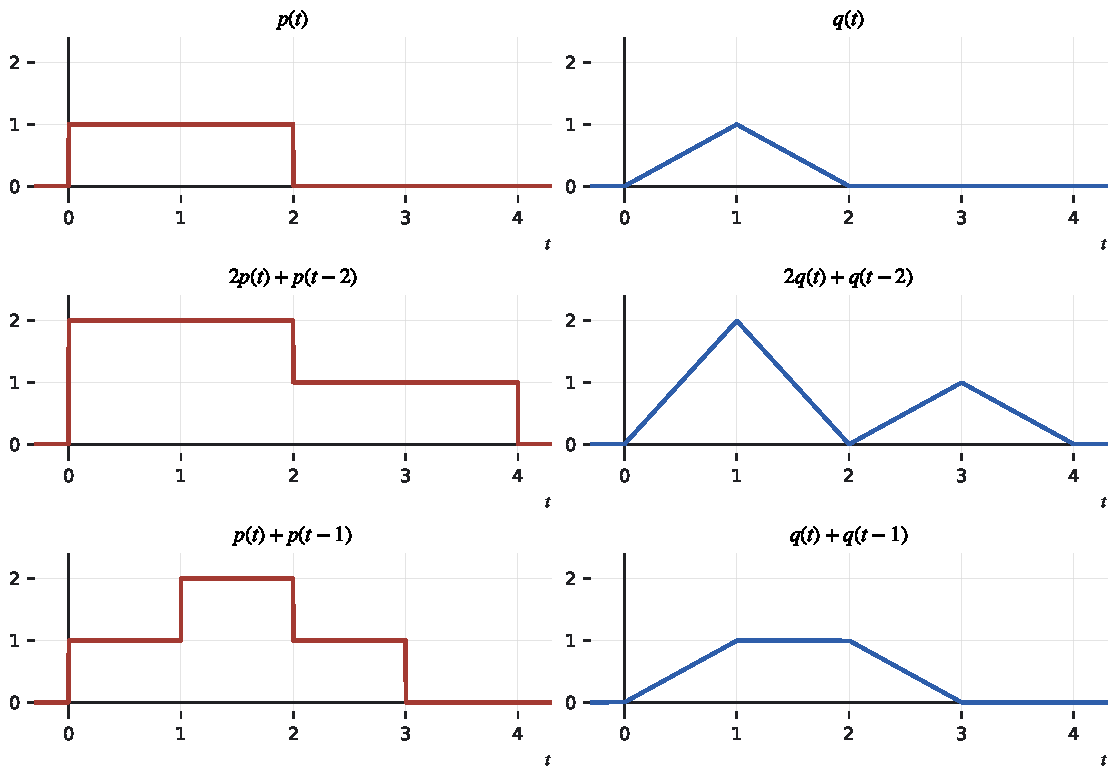
\includegraphics[width=0.88\textwidth]{04-convolution/examples/continuous-lti-superposition.pdf}
  \caption{已知矩形输入的三角响应后，逐项缩放、时移并叠加，得到两种组合输入的响应。}
  \label{fig:continuous-lti-superposition}
\end{figure}

连续时间 LTI 系统也可由\keyterm{单位冲激响应}完全描述。记
\begin{equation}
  \impulse(t)\longrightarrow\boxed{\text{连续时间 LTI 系统}}\longrightarrow h(t),
  \label{eq:continuous-impulse-response-flow}
\end{equation}
则移位、缩放的冲激满足
\[
  x(\tau)\impulse(t-\tau)
  \longrightarrow\boxed{\text{同一 LTI 系统}}\longrightarrow
  x(\tau)h(t-\tau).
\]

连续时间单位冲激 $\impulse(t)$ 是由积分作用定义的\red{广义函数}，不是 $t=0$ 处取“无穷大”的普通函数。为看清离散求和如何过渡到积分，先取宽度 $\Delta$、面积 $1$ 的窄脉冲
\[
  \impulse_\Delta(t)=
  \begin{cases}
    1/\Delta, & 0\leq t<\Delta,\\
    0, & \text{其他},
  \end{cases}
\]
并用它构造阶梯近似
\begin{equation}
  x_\Delta(t)
  =\sum_{k=-\infty}^{\infty}
  x(k\Delta)\impulse_\Delta(t-k\Delta)\Delta.
  \label{eq:continuous-step-approximation}
\end{equation}
\Cref{fig:continuous-impulse-approximation} 显示 $\Delta$ 变小时，单位面积窄脉冲变得更窄、更高。这里取的是积分作用的极限，不追问 $t=0$ 处的点值。

\begin{figure}[htbp]
  \centering
  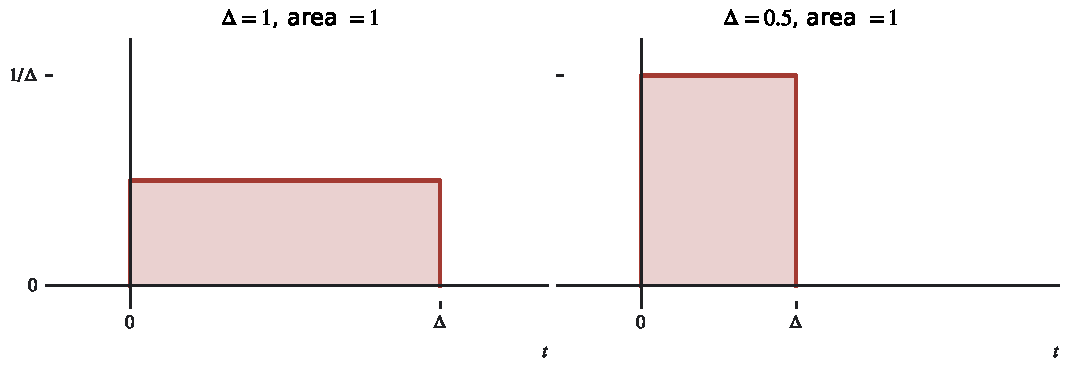
\includegraphics[width=0.76\textwidth]{04-convolution/continuous-impulse-approximation.pdf}
  \caption{单位面积窄脉冲 $\impulse_\Delta(t)$：宽度减半时，高度加倍。}
  \label{fig:continuous-impulse-approximation}
\end{figure}

设系统对 $\impulse_\Delta(t)$ 的响应为 $h_\Delta(t)$。对\cref{eq:continuous-step-approximation} 逐项使用线性与时不变性：
\[
  y_\Delta(t)=\sum_{k=-\infty}^{\infty}
  x(k\Delta)h_\Delta(t-k\Delta)\Delta.
\]
窄脉冲极限与系统响应的极限\blue{可以交换}时，$h_\Delta(t)$ 过渡到 $h(t)$，黎曼和过渡为积分：
\begin{equation}
  \boxed{
    y(t)=(x\conv h)(t)
    =\int_{-\infty}^{\infty}x(\tau)h(t-\tau)\dd\tau
  }.
  \label{eq:continuous-convolution-integral}
\end{equation}
右端称为\keyterm{卷积积分（convolution integral）}。图解仍按\hl{翻转、平移、相乘、积分}，最后一步由求和改成求面积。

\begin{remark}[离散与连续卷积的对应]
  两个公式结构相同：
  \[
    \begin{array}{c|c|c}
      & \text{基本分解} & \text{LTI 输出}\\ \hline
      \text{离散时间}
        & x[n]=\displaystyle\sum_k x[k]\impulse[n-k]
        & y[n]=\displaystyle\sum_k x[k]h[n-k]\\[6pt]
      \text{连续时间}
        & x(t)=\displaystyle\int x(\tau)\impulse(t-\tau)\dd\tau
        & y(t)=\displaystyle\int x(\tau)h(t-\tau)\dd\tau
    \end{array}
  \]
  区别只在连续时间由不可数多个移位冲激叠加，因此\red{求和换成积分}。
\end{remark}

\section{连续时间单位冲激的基本性质}
\label{sec:continuous-impulse-properties}

单位冲激由积分作用刻画，\red{峰值高度没有普通函数意义}。以下性质\blue{都按广义函数理解}。

\subsection{单位面积与抽样性质}

单位冲激满足
\begin{equation}
  \int_{-\infty}^{\infty}\impulse(t)\dd t=1.
  \label{eq:continuous-impulse-unit-area}
\end{equation}
只要积分区间内部包含 $0$，冲激积分就是 $1$；按相反方向跨过 $0$，积分为 $-1$；区间不含 $0$，积分为 $0$。

若 $x(t)$ 在 $t_0$ 附近连续，冲激会取出该处的值：
\begin{equation}
  \boxed{
    \int_{-\infty}^{\infty}x(t)\impulse(t-t_0)\dd t=x(t_0)
  }.
  \label{eq:continuous-impulse-sifting}
\end{equation}
取 $t_0=0$ 即得 $\int x(t)\impulse(t)\dd t=x(0)$。做含冲激的积分，判据是\hl{先找冲激位置}，\hl{再代入被抽样函数}。

\subsection{冲激与普通函数的乘积}

同样在广义函数意义下，若 $x(t)$ 在 $t_0$ 附近连续，则
\begin{equation}
  \boxed{
    x(t)\impulse(t-t_0)=x(t_0)\impulse(t-t_0)
  }.
  \label{eq:continuous-impulse-product}
\end{equation}
验证时两边乘任意连续函数 $\varphi(t)$ 并积分。由\cref{eq:continuous-impulse-sifting}，两边都得到
\[
  x(t_0)\varphi(t_0),
\]
所以它们对所有测试函数作用相同。计算时\red{只保留冲激位置处的函数值}，不能把 $\impulse(t-t_0)$ 当普通函数逐点约掉。

\begin{pitfall}[把单位冲激当成普通函数]
  “$\impulse(0)=\infty$，所以代入计算”不能定义冲激，也不能做可靠的代数运算。检查时回到单位面积与抽样性质：\red{冲激只在积分中集中权重}，结论由它对测试函数的作用决定。
\end{pitfall}

\subsection{尺度变换与复合函数中的冲激}

对任意非零实数 $a$，
\begin{equation}
  \boxed{
    \impulse(at)=\frac{1}{|a|}\impulse(t)
  },
  \qquad a\neq0.
  \label{eq:continuous-impulse-scaling}
\end{equation}
绝对值不能省略。$a<0$ 时，变量代换把积分上下限反向，刚好抵消微分中的负号；压缩或翻转冲激后都必须保持单位面积。更一般地，
\begin{equation}
  \impulse(at+b)
  =\frac{1}{|a|}\impulse\!\left(t+\frac{b}{a}\right).
  \label{eq:impulse-affine-scaling}
\end{equation}
判定时\hl{先求冲激位置}，\hl{再除以尺度绝对值}。

这个结论可推广到非线性复合。设 $f(t)$ 的实零点 $t_i$ 都是\blue{孤立的单零点}：
\[
  f(t_i)=0,
  \qquad
  f'(t_i)\neq0,
\]
且零点组成有限或可数集合，则
\begin{equation}
  \boxed{
    \impulse\bigl(f(t)\bigr)
    =\sum_{i}\frac{1}{|f'(t_i)|}\impulse(t-t_i)
  }.
  \label{eq:impulse-composite-function}
\end{equation}
每个零点附近用 $f(t)\approx f'(t_i)(t-t_i)$ 线性化，再套\cref{eq:continuous-impulse-scaling}。口诀是\hl{找全零点、代入导数、取绝对值}。

\begin{example}[二次多项式中的冲激]
  \label{eg:quadratic-composite-impulse}
  设 $f(t)=t^2-3t+2=(t-1)(t-2)$。零点为 $t_1=1$、$t_2=2$，且
  \[
    |f'(1)|=|-1|=1,
    \qquad
    |f'(2)|=|1|=1.
  \]
  因而
  \[
    \impulse(t^2-3t+2)=\impulse(t-1)+\impulse(t-2).
  \]
  右端冲激必须位于 $1$ 和 $2$。写成 $\impulse(t+1)+\impulse(t+2)$ 会把位置变成 $-1$ 和 $-2$，据此可立即发现符号错误。
\end{example}

\begin{pitfall}[忽略复合冲激公式的条件]
  \Cref{eq:impulse-composite-function} 要求零点是孤立单零点。若某处 $f(t_i)=0$ 且 $f'(t_i)=0$，\red{分母为零，局部线性化失效}；若 $f$ 在一段区间恒为零，\red{零点无法逐项编号}。这两种情形不能直接套用该式。
\end{pitfall}

\section{卷积的代数性质}
\label{sec:convolution-algebraic-properties}

\subsection{交换律}

\blue{只要相关求和或积分存在}，\red{离散与连续卷积都满足交换律}：
\begin{equation}
  \boxed{x\conv h=h\conv x}.
  \label{eq:convolution-commutativity}
\end{equation}
连续时间从
\[
  (x\conv h)(t)
  =\int_{-\infty}^{\infty}x(\tau)h(t-\tau)\dd\tau
\]
出发，令 $u=t-\tau$，则 $\dd u=-\dd\tau$；交换上下限后
\[
  (x\conv h)(t)
  =\int_{-\infty}^{\infty}h(u)x(t-u)\dd u
  =(h\conv x)(t).
\]
离散情形令 $m=n-k$ 即可。交换律说明计算时可以\hl{选择较容易翻转和平移的一项}，尽管推导 LTI 输出时 $h$ 有单位脉冲响应这一特殊身份。

\begin{remark}[单位脉冲响应决定 LTI 系统]
  若两个 LTI 系统的单位脉冲响应满足 $h_1=h_2$，则对任意适用输入 $x$，都有 $x\conv h_1=x\conv h_2$。在 LTI 前提下，相同的单位脉冲响应就是相同的输入输出关系。
\end{remark}

\subsection{结合律与串联系统}

只要相关求和或积分存在，并且允许交换求和或积分次序，卷积满足结合律：
\begin{equation}
  \boxed{
    (x\conv h_1)\conv h_2
    =x\conv(h_1\conv h_2)
  }.
  \label{eq:convolution-associativity}
\end{equation}
以连续时间为例，左端写成
\begin{align*}
  \bigl[(x\conv h_1)\conv h_2\bigr](t)
  &=\int_{-\infty}^{\infty}
    \left[\int_{-\infty}^{\infty}
      x(u)h_1(\tau-u)\dd u
    \right]h_2(t-\tau)\dd\tau\\
  &=\int_{-\infty}^{\infty}x(u)
    \left[\int_{-\infty}^{\infty}
      h_1(\tau-u)h_2(t-\tau)\dd\tau
    \right]\dd u\\
  &=\bigl[x\conv(h_1\conv h_2)\bigr](t).
\end{align*}
第二步交换积分次序；\blue{交换次序要求积分绝对收敛}，否则这一步不成立。

结合交换律，两个 LTI 系统\red{串联时可以交换先后次序}：
\[
  x(t)\longrightarrow\boxed{h_1(t)}
  \longrightarrow\boxed{h_2(t)}\longrightarrow y(t),
  \qquad
  x(t)\longrightarrow\boxed{h_2(t)}
  \longrightarrow\boxed{h_1(t)}\longrightarrow y(t).
\]
两条链的总单位冲激响应分别为 $h_1\conv h_2$ 与 $h_2\conv h_1$，因而等效。判定串联系统时可以\red{先卷积各级冲激响应}，再与输入卷积；也可以选更容易计算的级次顺序。

\subsection{分配律与并联系统}

卷积对加法满足分配律：
\begin{equation}
  \boxed{
    x\conv(h_1+h_2)
    =x\conv h_1+x\conv h_2
  }.
  \label{eq:convolution-distributivity}
\end{equation}
离散情形同样成立。两个 LTI 系统并联、输出相加时，总单位脉冲响应为 $h_1+h_2$：
\[
  y=x\conv h_1+x\conv h_2=x\conv(h_1+h_2).
\]
因此，\red{串联对应卷积，并联对应相加}。这也是把复杂 LTI 网络逐级化简为单个等效单位脉冲响应的基本规则。

\section{单位冲激的逼近表示}
\label{sec:impulse-approximations}

单位冲激可由多种普通函数族在广义函数意义下逼近。除了\cref{eq:continuous-step-approximation} 的单边窄脉冲，也可用关于原点对称、宽度 $\Delta$、高度 $1/\Delta$ 的矩形脉冲。只要对每个测试函数 $\varphi$ 都有
\[
  \lim_{\Delta\to0}
  \int_{-\infty}^{\infty}\varphi(t)\impulse_\Delta(t)\dd t
  =\varphi(0),
\]
就可写成 $\impulse_\Delta\to\impulse$。判据是\red{极限后的积分作用等于在零点抽样}；脉冲图形本身无需逐点收敛。

另一组重要的逼近是
\begin{equation}
  \boxed{
    \lim_{\Omega\to\infty}
    \frac{\sin(\Omega t)}{\pi t}
    =\impulse(t)
  }
  \quad\text{（广义函数意义）}.
  \label{eq:sinc-impulse-limit}
\end{equation}
在适当的测试函数条件下，
\[
  \lim_{\Omega\to\infty}
  \int_{-\infty}^{\infty}
  \varphi(t)\frac{\sin(\Omega t)}{\pi t}\dd t
  =\varphi(0).
\]
\Cref{fig:sinc-impulse-sequence} 显示主瓣随 $\Omega$ 增大而变窄、峰值升高，旁瓣快速振荡。这里取\red{广义函数意义的极限}，判断依据仍是它对测试函数的积分作用。

\begin{figure}[htbp]
  \centering
  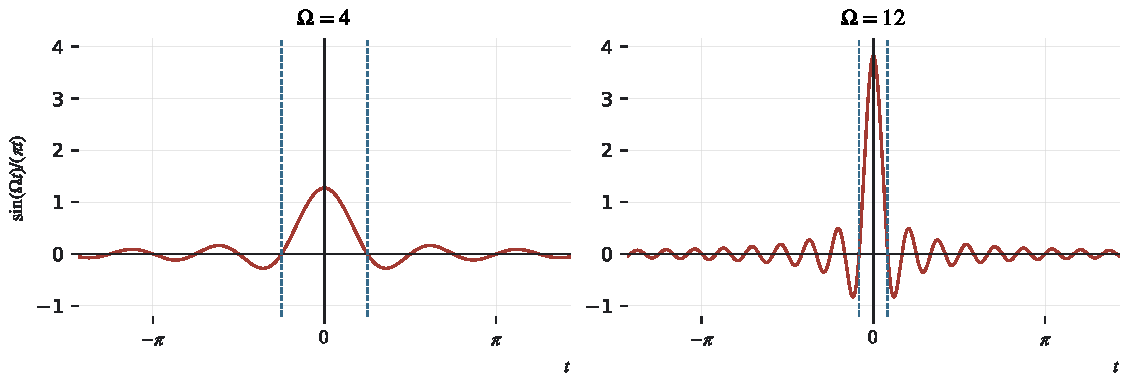
\includegraphics[width=0.84\textwidth]{04-convolution/sinc-impulse-sequence.pdf}
  \caption{冲激逼近 $\sin(\Omega t)/(\pi t)$；$\Omega$ 增大时主要积分贡献向原点集中。}
  \label{fig:sinc-impulse-sequence}
\end{figure}

\subsection{冲激逼近结论的验证}

下面说明\cref{eq:sinc-impulse-limit} 为什么在积分作用下成立。设测试函数 $\varphi$ 在原点附近连续可微、整体分段光滑，支撑包含在 $[-R,R]$ 内。由狄利克雷积分
\begin{equation}
  \lim_{\Omega\to\infty}
  \int_{-R}^{R}\frac{\sin(\Omega t)}{\pi t}\dd t=1,
  \label{eq:truncated-dirichlet-integral}
\end{equation}
把待验证的积分拆成
\begin{align*}
  \int_{-\infty}^{\infty}
  \varphi(t)\frac{\sin(\Omega t)}{\pi t}\dd t
  &={}
  \int_{-R}^{R}
  \frac{\varphi(t)-\varphi(0)}{\pi t}\sin(\Omega t)\dd t \\
  &\quad+
  \varphi(0)
  \int_{-R}^{R}\frac{\sin(\Omega t)}{\pi t}\dd t.
\end{align*}
令
\[
  q(t)=
  \begin{cases}
    \dfrac{\varphi(t)-\varphi(0)}{\pi t}, & t\neq0,\\[6pt]
    \dfrac{\varphi'(0)}{\pi}, & t=0,
  \end{cases}
\]
则 $q$ 在 $[-R,R]$ 上可积。由黎曼--勒贝格引理，第一项随 $\Omega\to\infty$ 趋于 $0$；由\cref{eq:truncated-dirichlet-integral}，第二项趋于 $\varphi(0)$。因此
\[
  \lim_{\Omega\to\infty}
  \int_{-\infty}^{\infty}
  \varphi(t)\frac{\sin(\Omega t)}{\pi t}\dd t
  =\varphi(0),
\]
所得结果\red{与单位冲激的抽样作用相同}。证明的关键是先减去零点值，再用振荡抵消剩余项。

\begin{remark}[黎曼--勒贝格引理]
  若 $q$ 可积，则它与越来越高频的正弦或余弦相乘后积分趋于零。正负振荡在短区间内不断抵消，于是不含 $\varphi(0)$ 的部分被消去。
\end{remark}

\section{常用卷积关系}
\label{sec:common-convolution-relations}

\subsection{矩形脉冲的阶跃表示}

位于 $[a,b)$、高度为 $1$ 的矩形脉冲可写成
\begin{equation}
  p(t)=\stepfun(t-a)-\stepfun(t-b),
  \qquad a<b.
  \label{eq:rectangle-step-representation}
\end{equation}
端点直接编码在两个阶跃的跳变位置中，\red{便于平移、求导和卷积}。高度为 $A$ 时，整体乘 $A$。

\begin{example}[两个错位矩形脉冲的卷积]
  设
  \[
    x(t)=\stepfun(t-1)-\stepfun(t-3),
    \qquad
    h(t)=\stepfun(t+1)-\stepfun(t-1).
  \]
  两个矩形宽度均为 $2$，支撑分别为 $[1,3]$ 与 $[-1,1]$。$x(\tau)$ 不动，翻转平移后 $h(t-\tau)$ 在 $[t-1,t+1]$ 上为 $1$。端点接触给出输出范围 $[0,4]$，两区间在 $t=2$ 时完全重合：
  \[
    \begin{array}{c|c|c}
      t\text{ 的范围}&\text{重叠区间}&(x\conv h)(t)\\ \hline
      t<0&\text{无}&0\\
      0\le t\le2&[1,t+1]&\displaystyle\int_1^{t+1}1\times1\dd\tau=t\\
      2<t\le4&[t-1,3]&\displaystyle\int_{t-1}^{3}1\times1\dd\tau=4-t\\
      t>4&\text{无}&0
    \end{array}
  \]
  合并各段：
  \[
    (x\conv h)(t)=
    \begin{cases}
      t, & 0\leq t\leq2,\\
      4-t, & 2<t\leq4,\\
      0, & \text{其他}.
    \end{cases}
  \]
  输出是支撑在 $[0,4]$、峰值为 $2$、峰值位置 $t=2$ 的三角脉冲。计算前用“左右端点相加”先定输出支撑。
\end{example}

\subsection{与单位阶跃卷积：积分器与累加器}

连续时间信号与单位阶跃卷积：
\begin{equation}
  (x\conv\stepfun)(t)
  =\int_{-\infty}^{t}x(\tau)\dd\tau.
  \label{eq:convolution-with-step-continuous}
\end{equation}
所以单位冲激响应为 $\stepfun(t)$ 的 LTI 系统是从 $-\infty$ 起算的积分器。离散时间对应
\begin{equation}
  (x\conv\stepfun)[n]
  =\sum_{k=-\infty}^{n}x[k],
  \label{eq:convolution-with-step-discrete}
\end{equation}
即\keyterm{累加器}。记忆判据是\red{阶跃把上限截到当前时刻}；实际计算仍要从阶跃条件求积分或求和范围。

\subsection{冲激偶与卷积求导}

单位冲激的一阶导数称为\keyterm{冲激偶（impulse doublet）}：
\begin{equation}
  \impulse'(t)=\frac{\dd\impulse(t)}{\dd t}.
  \label{eq:impulse-doublet-definition}
\end{equation}
它按对测试函数的作用定义。若 $x$ 在 $t_0$ 附近可微，分部积分给出
\begin{equation}
  \boxed{
    \int_{-\infty}^{\infty}
    x(t)\impulse'(t-t_0)\dd t
    =-x'(t_0)
  }.
  \label{eq:impulse-doublet-sifting}
\end{equation}
\red{负号来自分部积分，不能遗漏}。令 $x(t)=1$，立即得到
\begin{equation}
  \int_{-\infty}^{\infty}\impulse'(t)\dd t=0.
  \label{eq:impulse-doublet-zero-area}
\end{equation}
冲激偶的正、负作用相互抵消。判断时抓住\red{冲激抽样函数值，冲激偶抽样负导数}。

\blue{在适当的可微与收敛条件下}，卷积的导数可作用到任一因子：
\begin{equation}
  \boxed{
    \frac{\dd}{\dd t}(x\conv h)
    =x'\conv h
    =x\conv h'
  }.
  \label{eq:differentiation-of-convolution}
\end{equation}
特别地，$x\conv\impulse'=x'$。单位冲激响应为 $\impulse'(t)$ 的 LTI 系统就是理想微分器。

\subsection{卷积中的时移合成}

若两个卷积因子分别平移 $a$ 与 $b$，则
\begin{equation}
  x(t-a)\conv h(t-b)
  =(x\conv h)(t-a-b).
  \label{eq:convolution-shift-composition}
\end{equation}
两项时移量在输出端相加。取 $a=-t_0$、$b=t_0$，两项抵消：
\begin{equation}
  x(t+t_0)\conv h(t-t_0)=x(t)\conv h(t)
  \label{eq:opposite-shifts-cancel}
\end{equation}
口诀是\red{卷积两端的时移量相加}，不能把卷积当成逐点乘法。

\begin{example}[乘积、积分与卷积不可混淆]
  对同一个 $x(t+2)$ 与 $\impulse(t-3)$，三种运算给出不同结果：
  \begin{align*}
    x(t+2)\impulse(t-3)
      &=x(5)\impulse(t-3),\\
    \int_{-\infty}^{\infty}x(t+2)\impulse(t-3)\dd t
      &=x(5),\\
    x(t+2)\conv\impulse(t-3)
      &=x(t-1).
  \end{align*}
  前两式由冲激在 $t=3$ 处抽样；第三式是与移位冲激卷积，把整个信号向右平移 $3$，所以 $x(t+2)$ 变为 $x(t-1)$。动笔前先辨认运算符：\red{乘积保留冲激，积分留下数值}，\red{卷积平移信号}。
\end{example}

\section{由单位脉冲响应判断 LTI 系统性质}
\label{sec:lti-properties-from-impulse-response}

\subsection{BIBO 稳定性的充要条件}

\begin{theorem}[LTI 系统的 BIBO 稳定判据]
  \label{thm:lti-bibo-impulse-response}
  连续时间 LTI 系统 BIBO 稳定，当且仅当
  \begin{equation}
    \int_{-\infty}^{\infty}|h(t)|\dd t<\infty.
    \label{eq:ct-lti-bibo-condition}
  \end{equation}
  离散时间 LTI 系统 BIBO 稳定，当且仅当
  \begin{equation}
    \sum_{n=-\infty}^{\infty}|h[n]|<\infty.
    \label{eq:dt-lti-bibo-condition}
  \end{equation}
\end{theorem}

充分性：若 $|x(t)|\leq M$，则
\begin{align*}
  |y(t)|
  &=\left|\int_{-\infty}^{\infty}h(\tau)x(t-\tau)\dd\tau\right|\\
  &\leq\int_{-\infty}^{\infty}|h(\tau)|\,|x(t-\tau)|\dd\tau\\
  &\leq M\int_{-\infty}^{\infty}|h(\tau)|\dd\tau<\infty.
\end{align*}
任何有界输入都产生有界输出。

必要性：对实值系统，取有界输入
\[
  x(t)=\operatorname{sgn}h(-t),
\]
$h(-t)=0$ 时令 $x(t)=0$。在 $t=0$ 处，
\[
  y(0)=\int_{-\infty}^{\infty}x(\tau)h(-\tau)\dd\tau
  =\int_{-\infty}^{\infty}|h(-\tau)|\dd\tau.
\]
系统稳定时右端必须有限，故 $h$ 绝对可积。离散情形把积分改为求和。因此判据是\red{连续看绝对可积，离散看绝对可和}。

\begin{pitfall}[只检查冲激响应是否有界]
  $h(t)$ 有界不足以保证稳定。$h(t)=\stepfun(t)$ 有界，但绝对积分发散；有界常值输入会使输出不断累积。\red{不要只看峰值}，要算整个 $|h|$ 的面积或样值绝对值之和。
\end{pitfall}

\subsection{因果性的充要条件}

\begin{theorem}[LTI 系统的因果判据]
  \label{thm:lti-causality-impulse-response}
  连续时间 LTI 系统因果，当且仅当
  \begin{equation}
    h(t)=0,
    \qquad t<0.
    \label{eq:ct-lti-causality-condition}
  \end{equation}
  离散时间 LTI 系统因果，当且仅当
  \begin{equation}
    h[n]=0,
    \qquad n<0.
    \label{eq:dt-lti-causality-condition}
  \end{equation}
\end{theorem}

充分性：在时刻 $t_0$，
\[
  y(t_0)=\int_{-\infty}^{\infty}x(\tau)h(t_0-\tau)\dd\tau.
\]
当 $\tau>t_0$ 时 $t_0-\tau<0$，由\cref{eq:ct-lti-causality-condition}，$h(t_0-\tau)=0$，所以
\begin{equation}
  y(t_0)=\int_{-\infty}^{t_0}x(\tau)h(t_0-\tau)\dd\tau.
  \label{eq:causal-lti-output-past-only}
\end{equation}
\red{输出只依赖当前及过去输入}，系统因果。

反过来，单位冲激 $\impulse(t)$ 在 $t<0$ 时尚未发生。因果系统在此之前不能产生由它引起的响应，而该响应正是 $h(t)$，故 $h(t)=0$（$t<0$）。离散同理。判定时只需检查\blue{冲激响应在零时刻之前是否为零}。

\begin{remark}[与第三章判据的关系]
  第三章判断一般系统的因果性与稳定性，要直接检查输入输出关系。对 LTI 系统，\red{只需检查单位脉冲响应}。本节两条定理给出时域判据，后面的变换域分析也会反复使用。
\end{remark}
